\documentclass[a4paper]{article}
\usepackage[a4paper, top=8mm, bottom=8mm, left=8mm, right=8mm]{geometry}
\usepackage{polyglossia}
\setdefaultlanguage[babelshorthands=true]{russian}
\setotherlanguage{english}

\usepackage{fontspec}
\setmainfont{FreeSerif}
\newfontfamily{\russianfonttt}[Scale=0.7]{DejaVuSansMono}

\usepackage[tiny, compact]{titlesec}
\usepackage{titling}
\setlength{\droptitle}{-1cm}
\pretitle{\begin{center}\begin{bfseries}\Large}
\posttitle{\par\end{bfseries}\end{center}}
\preauthor{\begin{center}\normalsize}
\postauthor{\par\end{center}\vspace{-1.8cm}}
\usepackage{hyperref}
\usepackage{bookmark}
\usepackage{csquotes}
\usepackage{enumitem}
\usepackage{graphicx}
\usepackage{amsmath}

\title{Реализация свёртки изображений на Python}
\author{Баринов Георгий Александрович}
\date{}

\begin{document}
\maketitle
\begin{flushright}
    Группа: \emph{\enquote{25.Б42-мм}} \\
    Кафедра: \emph{системного программирования} \\
    Научный руководитель: \emph{Пономарев Николай Алексеевич} \\
    Номер семестра практики: \emph{2}
\end{flushright}

\section{Введение}

Свёртка~--- это операция, которая постоянно используется при работе с изображениями. Она применяется для размытия, повышения резкости, выделения границ и других преобразований. Математически свёртка изображения $I$ с ядром $K$ размера $(2p+1) \times (2p+1)$ определяется как:
\[
(I * K)[i, j] = \sum_{m=-p}^{p} \sum_{n=-p}^{p} I[i+m,\, j+n] \cdot K[m, n]
\]

Ядро свёртки (фильтр)~--- это небольшая, обычно квадратная матрица коэффициентов, определяющая характер воздействия на изображение. В процессе свёртки ядро последовательно сдвигается по изображению, и для каждого положения вычисляется взвешенная сумма значений пикселей под ядром.

Пример ядра, выполняющего равномерное размытие (\texttt{blur\_3x3}):
\[
\frac{1}{9} \begin{pmatrix}
1 & 1 & 1 \\
1 & 1 & 1 \\
1 & 1 & 1
\end{pmatrix}
\]
В рамках учебной практики предлагается реализовать данную операцию на языке Python, а затем сравнить производительность полученной реализации с библиотекой OpenCV.

\section{Постановка задачи}

\textbf{Целью работы является} разработка программы свёртки изображений на языке Python, её тестирование и сравнение скорости работы с~библиотекой OpenCV.

\textbf{Задачи:}
\begin{itemize}
    \item Реализовать функцию свёртки, корректно обрабатывающую как одноканальные (полутоновые), так и трёхканальные (RGB) изображения.
    \item Реализовать четыре режима обработки края изображения:
    \begin{itemize}
        \item \verb|zero_method|~--- заполнение областей за краем нулевыми значениями.
        \item \verb|extend_method|~--- дублирование крайних пикселей (прижимание к границе).
        \item \verb|reflection_method|~--- зеркальное отражение пикселей относительно края.
        \item \verb|wrap_method|~--- циклическое (круговое) замыкание противоположных краев.
    \end{itemize}
    \item Сформировать набор стандартных ядер (фильтров) размерностью $3 \times 3$ и $5 \times 5$:
    \begin{itemize}
        \item \verb|blur_kernel| и~\verb|box_blur_5x5|~--- усредняющее размытие.
        \item \verb|gaussian_blur| и~\verb|gaussian_blur_5x5|~--- размытие по Гауссу.
        \item \verb|sharpness_kernel|~--- повышение резкости.
        \item \verb|emboss_kernel|~--- эффект тиснения.
        \item \verb|highlighting_vertical_borders| и~\verb|highlighting_horizontal_borders|~--- выделение контуров.
    \end{itemize}
    \item Покрыть реализацию тестами с использованием эталонных изображений.
    \item Провести экспериментальное исследование производительности и сравнить скорость работы с библиотекой OpenCV.
\end{itemize}

\section{Реализация}

\subsection{Перевод в оттенки серого}

Функция \verb|rgb_to_grayscale| переводит RGB-изображение в одноканальное (оттенки серого) по стандартной формуле яркости\footnote{Recommendation ITU-R BT.601. URL: \url{https://www.itu.int/rec/R-REC-BT.601/en} (дата обращения: 27.05.2026)}:
\[
Y = 0{,}299 \cdot R + 0{,}587 \cdot G + 0{,}114 \cdot B
\]

Коэффициенты соответствуют стандарту BT.601 и учитывают восприятие цветов человеком. Вычисления выполняются поэлементно на массиве NumPy без циклов.

\subsection{Алгоритм выполнения свёртки}

Вычисление свёртки реализовано в функции \texttt{apply\_convolution} и представляет собой покоординатный обход матрицы изображения скользящим окном. Процесс состоит из следующих основных этапов:

\begin{enumerate}
    \item Инициализируется пустая результирующая матрица того же размера, что и исходное изображение.
    \item Выполняется последовательный обход каждого пикселя кадра.
    \item Для каждого пикселя рассматривается локальная окрестность, размер которой соответствует размеру ядра свёртки.
    \item Если скользящее окно выходит за границы изображения, координаты пикселей динамически пересчитываются выбранным методом обработки краёв.
    \item Вычисляется сумма произведений значений пикселей окрестности на коэффициенты ядра, после чего итоговое значение записывается в результирующую матрицу.
\end{enumerate}

\subsection{Запуск программы}

Управление параметрами приложения (выбор входного файла, ядра свёртки, метода обработки границ и режима цветности) осуществляется через интерфейс командной строки. Взаимодействие реализовано на базе стандартной библиотеки \texttt{argparse}.

Пример команды для запуска обработки изображения:
\begin{verbatim}
uv run python -m src.main input.png -o output.png -k emboss -e zero -c
\end{verbatim}

Доступные аргументы командной строки:
\begin{itemize}
    \item \texttt{input} (позиционный аргумент)~--- имя или путь к исходному файлу изображения.
    \item \texttt{-o}, \texttt{-–output}~--- путь для сохранения полученного результата (если аргумент не передан, файл не сохраняется).
    \item \texttt{-k}, \texttt{-–kernel}~--- идентификатор применяемого ядра свёртки. По умолчанию используется \texttt{blur}.
    \item \texttt{-e}, \texttt{-–edge}~--- метод обработки границ изображения (\texttt{zero}, \texttt{reflect}, \texttt{extend}, \texttt{wrap}). По умолчанию используется \texttt{zero}.
    \item \texttt{-c}, \texttt{-–color}~--- флаг для активации режима полноцветной обработки RGB-изображения по всем каналам. При отсутствии данного флага изображение автоматически конвертируется в оттенки серого.
\end{itemize}

\section{Тестирование}

Для проверки корректности алгоритмов свёртки применено интеграционное тестирование с использованием эталонных файлов. В качестве эталонов используются изображения, полученные заранее с помощью библиотеки OpenCV и сохранённые в директорию \texttt{tests/golden\_images}.

Набор тестов покрывает два сценария: \texttt{test\_grayscale\_convolution} (одноканальные изображения) и \texttt{test\_rgb\_convolution} (полноцветная поканальная свёртка). Внутри каждого сценария параметрически перебирается матрица из 8 типов ядер и 3 режимов обработки границ (\texttt{zero}, \texttt{reflect}, \texttt{extend}). При проверке фильтра \texttt{emboss} учитывается заложенная в алгоритм логика: смещение яркости на $+128$, ограничение диапазона промежуточных результатов до $[0, 255]$ и приведение к типу \texttt{uint8}.

\section{Экспериментальное исследование производительности}
Скрипт \verb|benchmark_convolution.py| производит замеры времени выполнения для двух реализаций:
\begin{itemize}
    \item \textbf{Учебная реализация (Educational)}~--- функция на чистом Python с использованием массивов NumPy, написанная в рамках данной практики.
    \item \textbf{OpenCV}~--- эталонная функция \verb|cv2.filter2D|, написанная на C++ с применением низкоуровневых оптимизаций.
\end{itemize}

Для обеспечения чистоты эксперимента (исключения влияния задержек дискового ввода-вывода) тестовые изображения синтезировались случайным образом непосредственно в оперативной памяти. Тесты запускались на квадратных матрицах размерами от $128\times128$ до $2048\times2048$ пикселей. Применялись разные ядра (\verb|blur_3x3|, \verb|emboss_3x3|), режимы обработки границ (\verb|reflect|, \verb|zero|) и цветовые пространства (RGB и оттенки серого). Для сбора статистически значимых данных каждый замер повторялся 5 раз после предварительного \enquote{прогрева} системы.

Эксперименты проводились на системе со следующими характеристиками: 
\textit{процессор} Apple M3, \textit{ОЗУ} 16~ГБ, \textit{ОС} macOS 26.3.1.

Результаты экспериментального исследования производительности визуализированы с помощью скрипта \verb|visualization.py| и представлены на рисунке~\ref{fig:bench}.

\begin{figure}[ht]
    \centering
    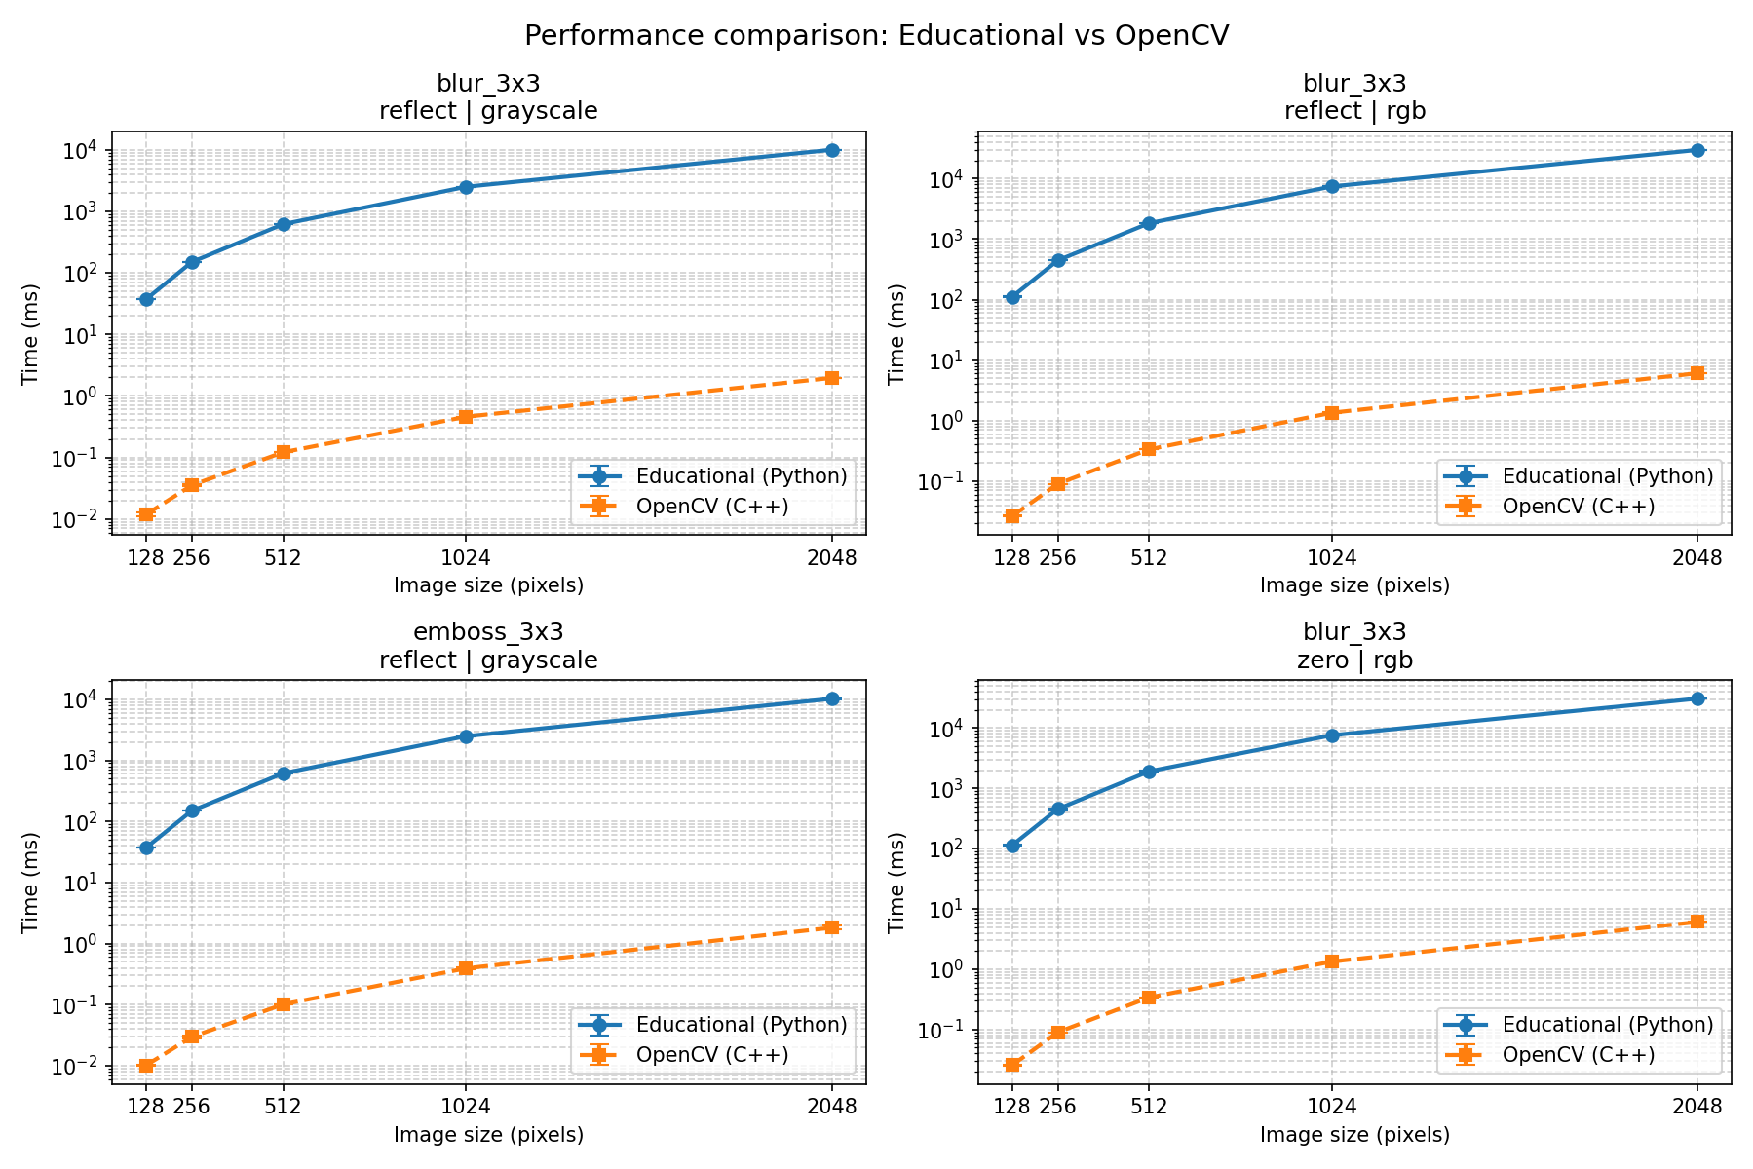
\includegraphics[width=\textwidth]{benchmark_results.pdf}
    \caption{Сравнение производительности библиотеки OpenCV и учебной реализации}
    \label{fig:bench}
\end{figure}

\subsection{Анализ результатов}

Как видно из полученных данных, алгоритмическая сложность обеих реализаций одинакова: время выполнения растёт строго пропорционально размеру изображения (количеству пикселей). Однако абсолютные показатели времени кардинально различаются.

Реализация на базе OpenCV отрабатывает в среднем в \textbf{4000--6000 раз быстрее} учебной реализации во всех сценариях. Столь значительный разрыв обусловлен тем, что Python является интерпретируемым языком, где каждая операция внутри вложенных циклов выполняется с большими накладными расходами, тогда как OpenCV написан на компилируемом C++.

\section{Заключение}

В ходе выполнения работы были решены поставленные задачи:
\begin{itemize}
    \item \textbf{Реализована функция свёртки}, корректно обрабатывающая как одноканальные (полутоновые), так и трёхканальные (RGB) изображения. В коде успешно реализованы четыре режима обработки границ: \verb|zero|, \verb|reflect|, \verb|extend| и \verb|wrap|.
    \item \textbf{Сформирован набор стандартных ядер свёртки} размерностью $3 \times 3$ и $5 \times 5$, включающий усредняющее размытие, размытие по Гауссу, повышение резкости, выделение вертикальных и горизонтальных контуров, а также фильтр тиснения (\texttt{emboss}) со специальной логикой яркостного сдвига на $+128$.
    \item \textbf{Программа покрыта тестами:} на базе фреймворка \texttt{pytest} реализовано интеграционное тестирование с использованием эталонных файлов. Попиксельное сравнение результатов с изображениями, обработанными библиотекой OpenCV, подтвердило математическую корректность разработанного алгоритма.
    \item \textbf{Проведено экспериментальное исследование производительности.} Эксперименты показали, что разработанная программа уступает OpenCV по скорости выполнения в 4000--6000 раз. Данный разрыв обоснован архитектурными особенностями: учебная реализация выполняет четыре уровня вложенных циклов на уровне интерпретатора Python, в то время как OpenCV работает на базе C++ кода с низкоуровневой оптимизацией.
\end{itemize}

Репозиторий с реализацией: \url{https://github.com/Gosha924/image-convolution-2-sem}.
\end{document}